\section{v1.1的重要修改内容:文献引用}
\textbf{2024年06月20日}:原版本的引用格式采用的是\textcolor{red}{顺序-编码制},与学校要求不符。本模板将引用格式修改为\textcolor{red}{著者-出版年制}。使用前置条件如下:
\subsection{制作或者生成bib文件}

\subsubsection{手动制作}
例如:
\begin{lstlisting}
@article{wanger2009,
	author    = {王二 and 张三 and 李四},
	key       = {wang2 er4 and zhang1 san1 & li3 si4},
	title     = {单引用测试,标题1},
	journal   = {journal},
	year      = {2010}	
	}
\end{lstlisting}
\begin{itemize}
	\item wanger2009:是文章的标签,引用时通过它,可以对应到文章。
	\item author:作者名称,不同作者按顺序用and分隔开。
	\item key:作者的拼音,数字表示声调。方便按拼音顺序排列参考文献
	\item title:文章标题
	\item journal:期刊名称
	\item year:出版年份
	...
\end{itemize}
不建议使用这种方式,挺麻烦的
\subsubsection{自动制作}
在阅读文献时使用zotero、endnote等文献管理器对文献进行管理,后期可以选中需要的文件一键导出参考文献的bib文件(如图\ref{参考文献导出示意图})。

\begin{figure}[h]
	\centering
	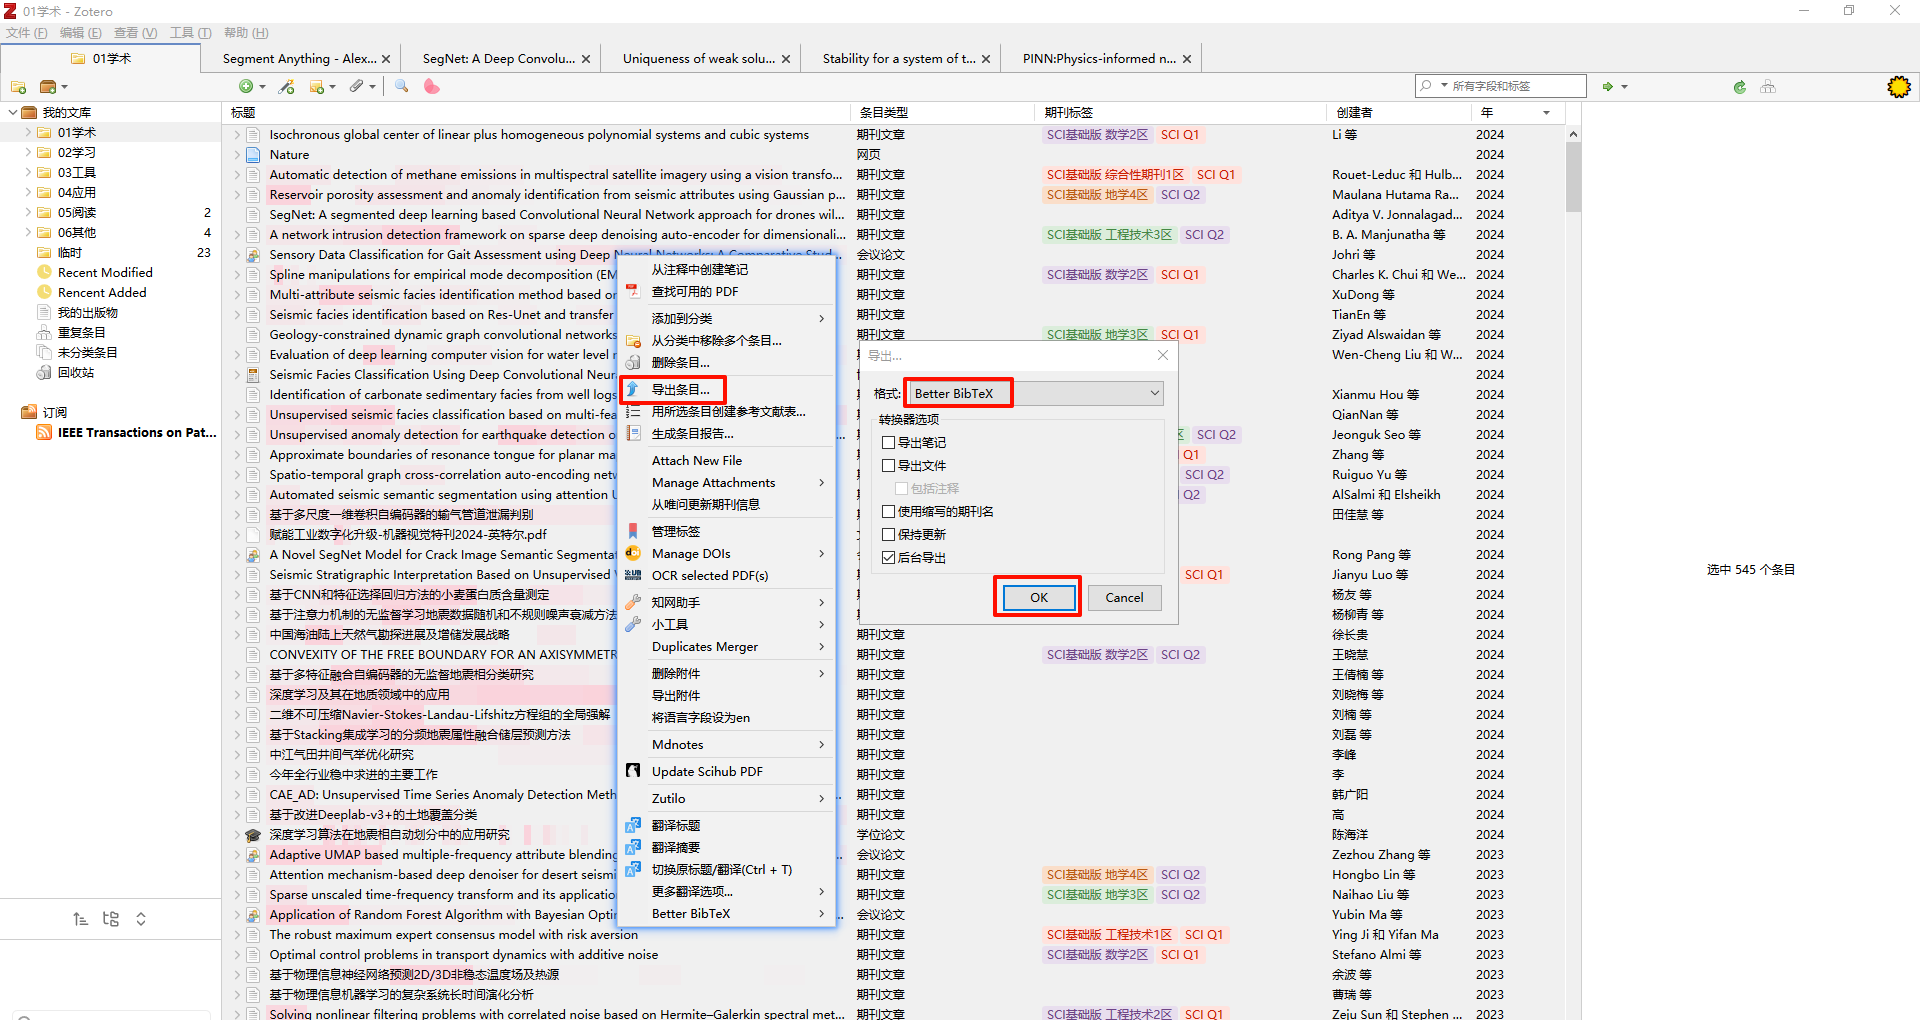
\includegraphics[width = 14cm]{figures/参考文献.png}
	\caption{zotero一键导出参考文献的bib文件}
	\label{参考文献导出示意图}
\end{figure}

\subsubsection{注意}
单独强调一下:无论是手动制作还是自动生成bib文件,只要是中文文献,就要手动加\textbf{key}值,以保证\textbf{中文文献在参考文献目录中能够按照拼音顺序排列}。例如:
\begin{lstlisting}
	@article{wanger2009,
		author    = {王二 and 张三 and 李四},
		key       = {wang2 er4 and zhang1 san1 & li3 si4},
	}
\end{lstlisting}
\subsection{两种引用格式}
有了bib文件,就可以在论文中插入引用了。假设最终需要引用的文献的bib文件如下:
\begin{lstlisting}
@article{wanger2009,
	author    = {王二 and 张三 and 李四},
	key       = {wang2 er4 and zhang1 san1 & li3 si4},
	title     = {单引用测试,标题1},
	journal   = {journal},
	year      = {2010}	
}
@article{zhangsan2010,
	author    = {张三 and 李四},
	key       = {zhang1 san1 & li3 si4},
	title     = {多引用测试,标题1},
	journal   = {journal},
	year      = {2010}	
}
@article{lisi2011,
	author    = {李四 and 张三},
	key       = {li3 si4 & zhang1 san1},
	title     = {多引用测试,标题2},
	journal   = {journal},
	year      = {2011}	
}
\end{lstlisting}
\subsubsection{第一种引用形式}
\textbf{示例1:}\cite{wanger2009}这是第一种引用形式。
\begin{lstlisting}
\cite{wanger2009}
\end{lstlisting}

\subsubsection{第二种引用形式}
\textbf{示例2:}这是第二种引用形式\citep{wanger2009}。
\begin{lstlisting}
\citep{wanger2009}
\end{lstlisting}

\textbf{示例3:}这是第二种引用形式\citep{wanger2009,zhangsan2010,lisi2011},引用多篇佐证本文观点。
\begin{lstlisting}
\citep{wanger2009,zhangsan2010,lisi2011}
\end{lstlisting}

写作时基本是用这两种引用形式,,英文文献与上面引用一致(会自动处理成英文版本)。

\textbf{示例4:}英文文献示例\citep{LiK2019}。
\begin{lstlisting}
\citep{LiK2019}
\end{lstlisting}


注意:只要bib文件是严格按照要求制作的,就不会在这里出现错误。所以最好学习使用文献管理器制作bib文件,而非手动制作。
\subsection{参考文献目录}

只要bib文件是严格正确的,参考文献目录会自动生成符合规定(中文在上,外文在下。文献名称按顺序排列下来等规则)的参考文献目录。所以这里不需要过多关注。

bib文件放在body文件夹中,其名称为:refer.bib。
\begin{lstlisting}
\phantomsection
\bibliography{body/refer.bib}
\end{lstlisting}
